\label{1.2.10}

\textit{The Cone Over a Projective Variety} (\ref{Fig. 1}). Let $Y \subseteq \P^n$ be a nonempty algebraic set, and let $\theta :\A^{n + 1} -
\{(0, \dots ,0)\} \longrightarrow \P^n$ be the map which sends the point with affine coordinates $(a_0, \dots, a_n)$ to the point with homogeneous coordinates $(a_0 , \dots ,a_n)$· We define the \textit{affine cone} over $Y$ to be

\[
    C(Y) = \theta^{- 1}[Y] \cup \{(0, \dots ,0)\}.
\]

\begin{enumerate}[label = (\alph*)]
    \item Show that $C(Y)$ is an algebraic set in $\A^{n + 1}$, whose ideal is equal to $I(Y)$, considered as an ordinary ideal in $k[x_0 , \dots x_n]$.
    
    \item $C(Y)$ is irreducible if and only if $Y$ is.
    
    \item $\dim C(Y) = \dim Y + 1$.
\end{enumerate}

Sometimes we consider the projective closure $\overline{C(Y)}$ of $C(Y)$ in $\P^{n + 1}$ . This is called the \textit{projective cone} over $Y$.

\newpage

\begin{figure}
    \centering
    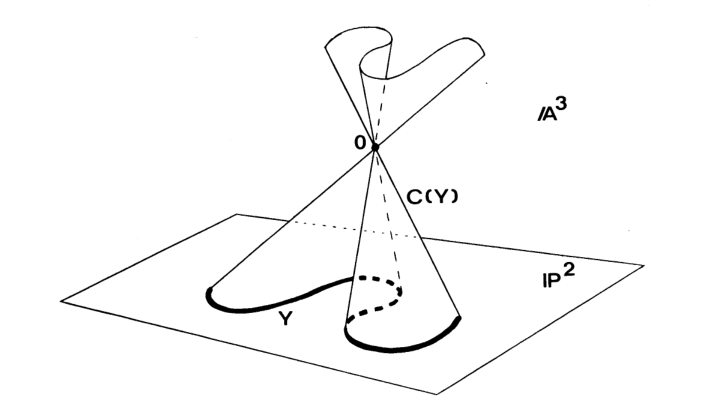
\includegraphics{Fig 01}
    \caption{The cone over a curve in $\P^2$.}
    \label{Fig. 1}
\end{figure}

\begin{proof}
    
\end{proof}